\documentclass{beamer}
\mode<presentation>
\usetheme{CambridgeUS}
\usepackage[russian]{babel}
\usepackage[utf8]{inputenc}
\usepackage[T2A]{fontenc}
\usepackage{sansmathaccent}

\usepackage{verbatim}
\usepackage{alltt}
\usepackage{minted}
\usepackage{amsmath}

\pdfmapfile{+sansmathaccent.map}
\title[Динамическое программирование]{Динамическое программирование}
\author{Наумов Д.А., доц. каф. КТ}
\date[13.09.2021] {Алгоритмы и структуры данных, 2021}

\begin{document}

%ТИТУЛЬНЫЙ СЛАЙД
\begin{frame}
  \titlepage
\end{frame}

\begin{frame}
  \frametitle{Содержание лекции}
  \tableofcontents
\end{frame}

\section{Введение в динамическое программирование}

\begin{frame}[t]
	Динамическое программирование, как правило, применяется к задачам оптимизации (optimization problems). Такая задача может иметь много возможных решений. С каждым вариантом решения можно сопоставить какое-то значение, и нам нужно найти среди них решение с оптимальным (минимальным или максимальным) значением.
	\begin{enumerate}
	    \item Описание структуры оптимального решения.
        \item Определение значения, соответствующего оптимальному решению, с использованием рекурсии.
        \item Вычисление значения, соответствующего оптимальному решению, обычно с помощью метода восходящего анализа.
        \item Составление оптимального решения на основе информации, полученной на
предыдущих этапах.
	\end{enumerate}
	Этапы 1-3 составляют основу метода динамического программирования для решения задач. Этап 4 может быть опущен, если требуется узнать только значение, соответствующее оптимальному решению.
\end{frame}

\section{Пример: разрезание стержня}

\begin{frame}[t]
    \begin{block}{Постановка задачи}
        Компания покупает длинные стальные стержни, режет их на куски и продает. Сама порезка стержней не стоит компании ни копейки. Руководство компании хочет знать, как лучше всего разрезать стержни на части.    
    \end{block}
	\begin{figure}[h]
		\centering
		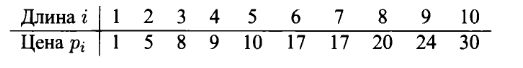
\includegraphics[scale=0.6]{images/lec09-pic01.png}
		\caption{Пример таблицы цен отрезков стержня}
	\end{figure}
	Имеются стержень длиной $n$ и таблица цен $p_i$ для $i = 1, 2, ..., n$. Необходимо найти максимальную прибыль $r_n$, получаемую при разрезании стержня и продаже полученных кусков. Если цена $p_n$ стержня длиной $n$ достаточно велика, оптимальное решение может состоять в продаже стержня целиком, без разрезов.
\end{frame}

\begin{frame}[t]{Разрезание стержня}
	\begin{figure}[h]
		\centering
		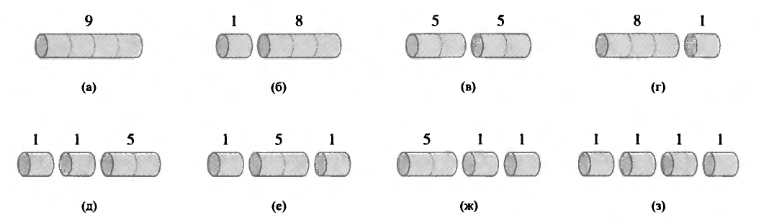
\includegraphics[scale=0.6]{images/lec09-pic02.png}
		\caption{Восемь способов разрезания стержня}
	\end{figure}
\end{frame}

\begin{frame}[t]{Разрезание стержня}
    Стержень длиной $n$ можно разрезать $2^{n-1}$ разными способами, поскольку мы можем независимо выбирать, резать его или нет на расстоянии $i$ от левого конца, где $i= 1,2,...,n-1$.
	\begin{figure}[h]
		\centering
		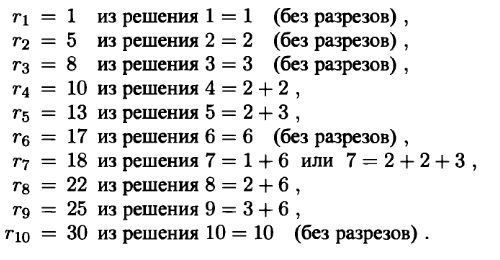
\includegraphics[scale=0.6]{images/lec09-pic03.png}
		\caption{Расчет максимальной прибыли}
	\end{figure}
\end{frame}

\begin{frame}[t]{Разрезание стержня}
    В общем случае можно записать значения $r_n$ для $n>1$ через оптимальные прибыли от более коротких стержней:
    \[r_n=max(p_n, r_1+r_{n-1}, r_2+r_{n-2},...,r_{n-1}+r_n)\]

    \begin{itemize}
        \item Первый аргумент, $p_n$ соответствует продаже стержня длиной $n$ как есть, без разрезов.
        \item Прочие $n-1$ аргументов функции $max$ соответствуют максимальным доходам, получаемым при первоначальном разрезании стержня на две части размерами $i$ и $n-i$, для каждого $i=1, 2,..., n-1$, с последующим оптимальным разрезанием второй части. 
    \end{itemize}
    
    Придется рассмотреть все возможные значения $i$ и выбрать из них то, которое максимизирует доход. 
    
    Кроме того, возможно, следует не выбирать ни одного значения $i$ вообще, а предпочесть продавать стержни неразрезанными.
\end{frame}

\begin{frame}[t]{Разрезание стержня}
    \begin{enumerate}
        \item Для решения исходной задачи размером $n$ мы решаем меньшие задачи того же вида. 
        \item Как только мы сделали первый разрез, мы можем рассматривать две части стержня как независимые экземпляры задачи разрезания стержня. 
        \item Общее оптимальное решение включает оптимальные решения двух связанных подзадач, максимизирующих доходы от каждой из двух частей стержня. 
    \end{enumerate}
    
    \begin{block}{Задача разрезания стержня}
        демонстрирует оптимальную подструктуру: оптимальное решение задачи включает оптимальные решения подзадач, которые могут быть решены независимо.
    \end{block}
\end{frame}

\begin{frame}[t]{Разрезание стержня}
    \begin{itemize}
        \item Мы рассматриваем разрезание стержня как состоящее из первой части длиной $i$ и остатка длиной $n-i$. Первая часть далее не разрезается; резать можно только остаток. 
        
        \item Таким образом, мы можем рассматривать любое разрезание стержня длиной $n$ как первую часть и некоторое разделение на части остатка стержня без первой части. 
    
        \item При этом допускается и решение без разрезов, если первая часть имеет размер $i=n$ и дает прибыль $r_n$, а остаток длиной $0$ дает нулевой доход. 
    \end{itemize}
    
    В итоге мы получаем более простую версию уравнения:
    \[r_n=max(r_i+r_{n-i}), i=1..n\]
\end{frame}

\begin{frame}[t]{Разрезание стержня}
    \begin{figure}[h]
		\centering
		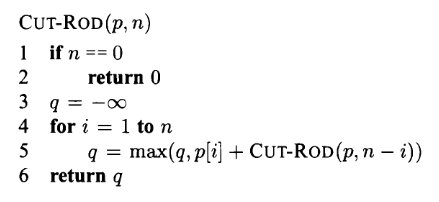
\includegraphics[scale=1.0]{images/lec09-pic04.png}
		\caption{Простой рекусивный способ вычислений}
	\end{figure}
\end{frame}

\begin{frame}[t]{Разрезание стержня}
    \begin{figure}[h]
		\centering
		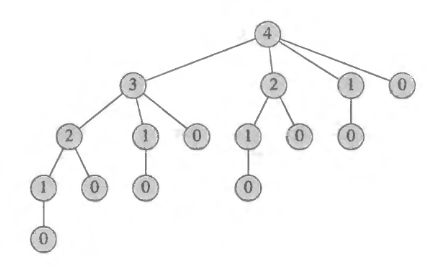
\includegraphics[scale=0.7]{images/lec09-pic05.png}
		\caption{Дерево рекурсии}
	\end{figure}
	
	Процедура явным образом рассматривает все $2^{n-1}$ возможных способа разрезания стержня длиной $n$.
\end{frame}

\begin{frame}[t]{Разрезание стержня}
    \begin{itemize}
        \item Имеющееся рекурсивное решение неэффективно из-за того, что многократно решаются одни и те же подзадачи, мы будем сохранять их решения, тем самым добиваясь только однократного решения подзадач.
    
        \item Если позже нам вновь придется решать такую подзадачу, мы просто найдем ее ответ, не решая ее заново. 
    
        \item Таким образом, динамическое программирование использует дополнительную память для экономии времени вычисления; это один из примеров \textbf{пространственно-временного компромисса}.
    \end{itemize}
\end{frame}

\begin{frame}[t]{Нисходящая рекурсия}
    \begin{block}{Нисходящая рекурсия с запоминанием}
        \begin{enumerate}
            \item При таком подходе мы пишем процедуру рекурсивно, как обычно, но модифицируем ее таким образом, чтобы она запоминала решение каждой подзадачи (обычно в массиве или хеш-таблице). 
            \item Теперь процедура первым делом проверяет, не была ли эта задача решена ранее. Если была, то возвращается сохраненное значение (и экономятся вычисления на данном уровне). 
            \item Если же подзадача еще не решалась, процедура вычисляет возвращаемое значение, как обычно. Мы говорим, что данная рекурсивная процедура с запоминанием — она запоминает вычисленный ею результат.
        \end{enumerate}
    \end{block}
\end{frame}

\begin{frame}[t]{Разрезание стержня}
    \begin{figure}[h]
		\centering
		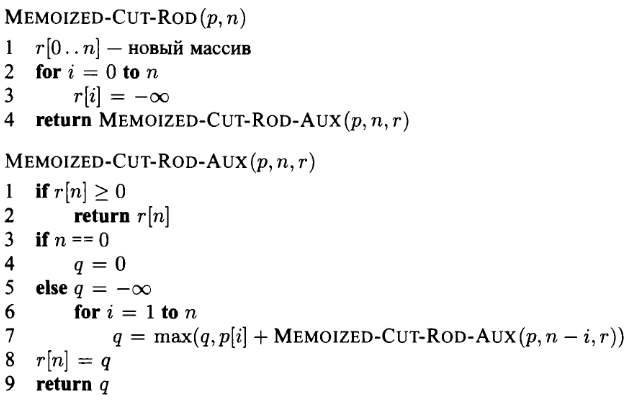
\includegraphics[scale=0.6]{images/lec09-pic06.png}
		\caption{Нисходящий подход}
	\end{figure}
\end{frame}

\begin{frame}[t]{Восходящий подход}
    \begin{block}{Восходящий подход}
        \begin{enumerate}
            \item Восходящий подход зависит от некоторого естественного понятия “размера” подзадачи, такого, что решение любой конкретной подзадачи зависит только от решения “меньших” подзадач. 
            \item Мы сортируем подзадачи по размерам в возрастающем порядке. При решении определенной подзадачи необходимо решить все меньшие подзадачи, от которых она зависит, и сохранить полученные решения. 
            \item Каждую подзадачу мы решаем только один раз, и к моменту, когда мы впервые с ней сталкиваемся, все необходимые для ее решения подзадачи уже решены.
        \end{enumerate}     
    \end{block}
\end{frame}

\begin{frame}[t]{Разрезание стержня}
    \begin{figure}[h]
		\centering
		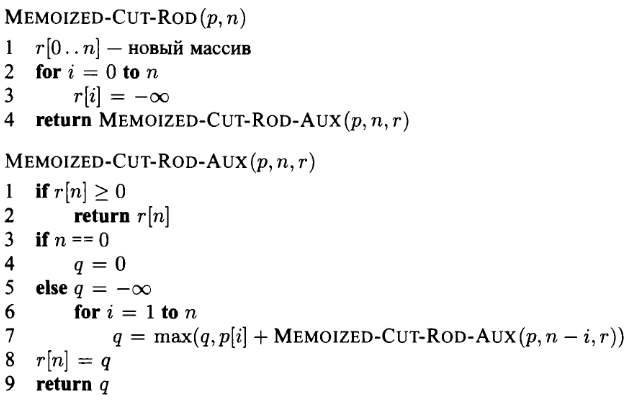
\includegraphics[scale=0.6]{images/lec09-pic06.png}
		\caption{Восходящий подход}
	\end{figure}
\end{frame}

\begin{frame}[t]
    \begin{block}{Граф подзадач}
        ориентированный граф, содержащий по одной вершине для каждой из различных подзадач.
    \end{block}
    Граф подзадач содержит дугу, идущую от вершины подзадачи х к вершине подзадачи у, если определение оптимального решения подзадачи х непосредственно включает поиск оптимального решения для подзадачи у.   
   \begin{figure}[h]
		\centering
		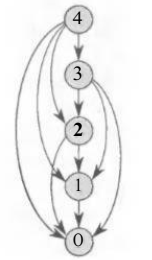
\includegraphics[scale=0.6]{images/lec09-pic08.png}
	\end{figure}
\end{frame}

\begin{frame}[t]{Восстановление решения}
    Можно расширить подход динамического программирования и записывать не только вычисленное оптимальное значение каждой подзадачи, но и выбор, который приводит к этому оптимальному значению. 
    \begin{figure}[h]
		\centering
		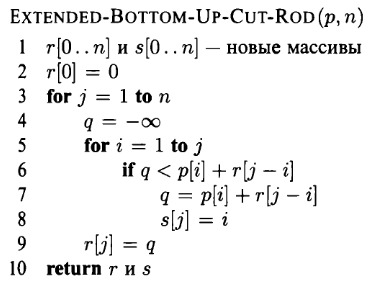
\includegraphics[scale=0.6]{images/lec09-pic09.png}
	\end{figure}
\end{frame}

\begin{frame}[t]{Восстановление решения}
   \begin{figure}[h]
		\centering
		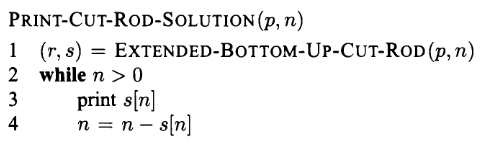
\includegraphics[scale=0.7]{images/lec09-pic10.png}
	\end{figure}
	
   \begin{figure}[h]
		\centering
		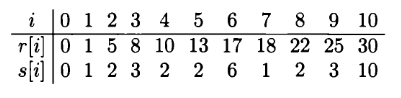
\includegraphics[scale=0.7]{images/lec09-pic11.png}
		\caption{Результаты работы алгоритмов}
	\end{figure}	
\end{frame}

\section{Пример: Перемножение цепочки матриц}

\begin{frame}[t]{Постановка задачи 2: перемножение матриц}
    Пусть имеется последовательность (цепочка) 
    \[
    A_1, A_2,...,A_n, 
    \]
    состоящая из $n$ матриц, и нужно вычислить их произведение.
    
    ~
    
    Если задана последовательность четырех матриц, то способ вычисления их произведения можно полностью определить с помощью скобок пятью разными способами:
   \begin{figure}[h]
		\centering
		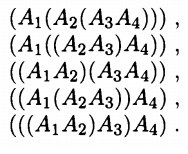
\includegraphics[scale=0.6]{images/lec09-pic12.png}
	\end{figure}
\end{frame}

\begin{frame}[t]{Постановка задачи}
    \begin{figure}[h]
		\centering
		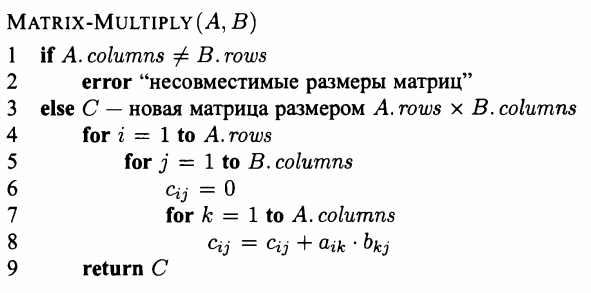
\includegraphics[scale=0.6]{images/lec09-pic13.png}
	\end{figure}
	
	Если $A$ — это матрица размером $p x q$, а $B$ — матрица размером $q x r$, то в результате их перемножения получится матрица $C$ размером $р х r$.

    Время вычисления матрицы $С$ преимущественно определяется количеством произведений скаляров,  которое равно $p\cdot q\cdot r$.
\end{frame}

\begin{frame}[t]{Постановка задачи}
	От того, как расставлены скобки при перемножении последовательности матриц, может сильно зависеть время, затраченное на вычисление произведения.
	
	\[A_1(10, 100)\]
	\[A_2(100, 5)\]
	\[A_3(5, 50)\]
	
	Определить количество операций умножения для двух вариантов расстановки скобок.
\end{frame} 

\begin{frame}[t]
    Для заданной последовательности $n$ матриц $A_1, A_2,...,A_n$, в которой матрица $A_i, i=1..n$, имеет размер $р_{i-1} х р_i$, с помощью скобок следует полностью определить порядок умножений, при котором количество скалярных умножений сведется к минимуму.
    
    \begin{block}{Подсчет количества способов расстановки скобок}
        \begin{equation*}
            P(n) = 
            \begin{cases}
                1, &\text{если n=1}\\
                \sum_{л=1}^{n-1}P(k)P(n-k) &\text{если n>=2}
            \end{cases}
        \end{equation*}
    \end{block}
	\begin{enumerate}
	    \item Описание структуры оптимального решения.
        \item Определение значения, соответствующего оптимальному решению, с использованием рекурсии.
        \item Вычисление значения, соответствующего оптимальному решению, обычно с помощью метода восходящего анализа.
        \item Составление оптимального решения на основе информации, полученной на
предыдущих этапах.
	\end{enumerate}    
\end{frame}

\begin{frame}[t]{1. Структура оптимальной расстановки скобок}
    Обозначим для удобства результат перемножения матриц $A_i A_{i+1}...A_j$ через $A_{i..j}$, где $i < j$. 
    
    ~
    
    Заметим, что если задача нетривиальна, т.е. $i<j$, то любой способ расстановки скобок в произведении $A_i\cdot ... \cdot A_j$ разбивает это произведение между матрицами $A_k$ и $A_{k+1}$, где $k$ - целое, удовлетворяющее условию $i<k<j$.
    
    ~
    
    Таким образом, при некотором $k$ сначала выполняется вычисление матриц $A_{i..k}$ и и $A_{k_j}$, а затем они умножаются друг на друга, в результате чего получается произведение $A_{i..j}$. 
    
    ~
    
    Стоимость, соответствующая этому способу расстановки скобок, равна сумме стоимости вычисления матриц $A_{i..k}$, $A_{k_j}$ и их произведения.    
\end{frame}

\begin{frame}[t]{2. Рекурсивное решение}
    Путь $m[i,j]$  - минимальное количество скалярных умножений, необходимых для вычисления матрицы $A_{i..j}$. 
    
    Тогда в полной задаче минимальная стоимость матрицы $А_{1..n}$ равна $m[1,n]$.
    \[
    m[i,j] = m[i,k] + m[к+1,j] + p_{i-1}p_kp_j
    \]
    В этой рекурсивной формуле предполагается, что значение $k$ известно, но на самом деле это не так. Для выбора этого значения всего имеется $j-i$ возможностей - $k=i,i+1,...,j$.
    
    \begin{equation*}
            m[i,j] = 
            \begin{cases}
                0, &\text{если i=j}\\
                \min(m[i,k]+m[k+1,j+p_{i-1}p_kp_j), i<=k<=j &\text{если i<j}
            \end{cases}
    \end{equation*}
    
    Обозначим через $s[i,j]$ значение $k$, в котором последовательность $A_{i..j}$ разбивается на две подпоследовательности в процессе оптимальной расстановки скобок.
\end{frame}

\begin{frame}[t]{3. Вычисление оптимальных стоимостей}
    Размеры матриц $A_i$ равны $p_{i-1} x p_i (i=1, 2,..., n)$. 
    
    ~
    
    Входные данные представляют собой последовательность 
    $p = (p_0, p_1,..., p_n)$, длина данной последовательности равна $n+1$. 
    
    ~
    
    В процедуре используется вспомогательная таблица $m[1..n,1..n]$ для хранения стоимостей $m[i, j]$ и вспомогательная таблица $s[1..n,1..n]$, в которую заносятся индексы $k$, при которых достигаются оптимальные стоимости $m[i,j]$.
    
    ~
    
    При $k=i,i+1,..,j-1$ матрица $A_{i..k}$ представляет собой произведение $k-i+1<j-i+1$ матриц, а матрица $A_{k..j}$ - произведение $j-к<j-i+1$ матриц. Таким образом, в ходе выполнения алгоритма следует организовать заполнение таблицы $m$ в порядке возрастания длин последовательностей матриц. 
\end{frame}

\begin{frame}[t]
   \begin{figure}[h]
		\centering
		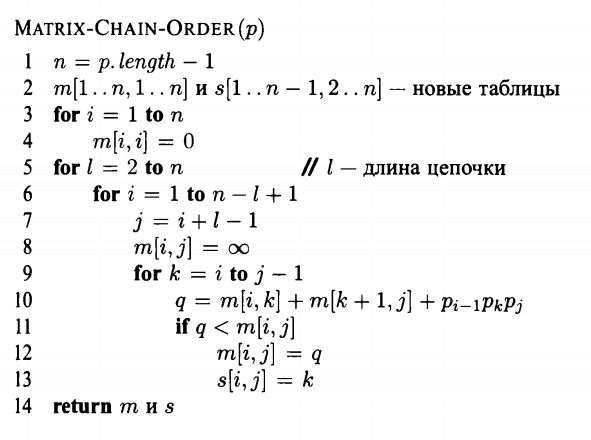
\includegraphics[scale=0.6]{images/lec09-pic14.png}
	\end{figure}
\end{frame}

\begin{frame}[t]
   \begin{figure}[h]
		\centering
		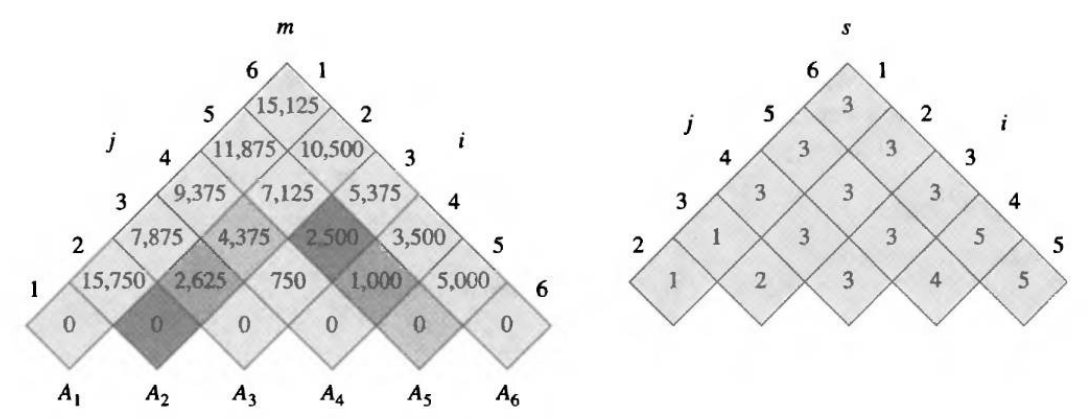
\includegraphics[scale=0.35]{images/lec09-pic15.png}
		\caption{Вычисленные значения таблиц m и s (n=6) для Matrix-Change-Order}
	\end{figure}
	
    \begin{figure}[h]
		\centering
		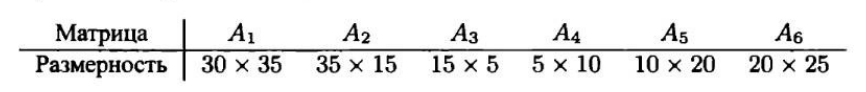
\includegraphics[scale=0.35]{images/lec09-pic16.png}
	\end{figure}
	
    \begin{figure}[h]
		\centering
		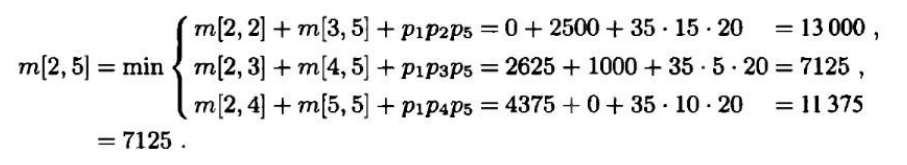
\includegraphics[scale=0.35]{images/lec09-pic17.png}
	\end{figure}	
\end{frame}

\begin{frame}[t]{4. Построение оптимального решения}
    Оптимальное вычисление произведения матриц $A_{1..n}$ выглядит как 
$A_{1..s[1,n]} A_{s[1,n+1]..n}$.

    ~
    
    Все предшествующие произведения матриц можно вычислить рекурсивно, поскольку элемент $s[1,s[1,n]]$ определяет матричное умножение, выполняемое последним при вычислении при вычислении $A_{1..s[1,n]}$ , a
    $s[s[1,n]+1, n]$ - последнее умножение при вычислении $A_{s[1,n]+1..n}$.
\end{frame}

\begin{frame}[t]{4. Построение оптимального решения}
    \begin{figure}[h]
		\centering
		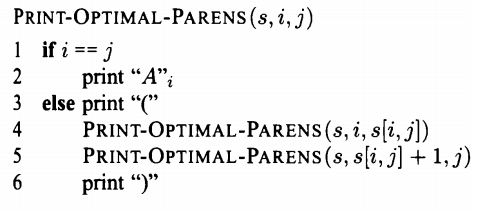
\includegraphics[scale=0.75]{images/lec09-pic18.png}
	\end{figure} 
	
	Результат вызова процедуры Print-Optimal-Parens(s, 1, 6):
	
	\[((A_1(A_2A_3))((A_4A_5)A_6))\]
\end{frame}

\end{document}
